
%(BEGIN_QUESTION)
% Copyright 2006, Tony R. Kuphaldt, released under the Creative Commons Attribution License (v 1.0)
% This means you may do almost anything with this work of mine, so long as you give me proper credit

En oljesump i et hydraulikksystem har en flottørbasert nivåbryter for å registrere lavt oljenivå og gi automatisk nedstenging av hydraulikksystemet:

$$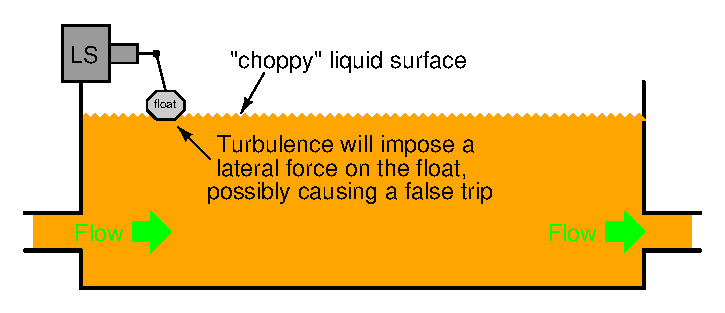
\includegraphics[width=15.5cm]{i00298x01.eps}$$

Oljestrømmen gjennom sumpen er høy, og dette gir et problem.  Med så turbulent olje ligger ikke flottøren rolig på overflaten.  I stedet kastes den rundt på den urolige overflaten, noe som kan få nivåbryteren til å ``tro'' flottøren har gått lengre ned enn den faktisk har, og dermed gi unødvendige nedstenginger.

En løsning er \textit{stilling well}.  Beskriv hva et ``stilling well'' er, hvordan du kan lage ett for denne applikasjonen, og hvorfor det virker.

\vskip 20pt \vbox{\hrule \hbox{\strut \vrule{} {\bf Forslag til sokratisk diskusjon} \vrule} \hrule}

\begin{itemize}
\item{} Ville en ultralyd-nivåbryter vært immun mot turbulensen?  Forklar hvorfor eller hvorfor ikke.
\end{itemize}

\underbar{file i00298}
%(END_QUESTION)





%(BEGIN_ANSWER)

Jeg lar deg finne selve løsningen på denne!

%(END_ANSWER)





%(BEGIN_NOTES)

Et \textit{stilling well} er et vertikalt rør plassert i prosessvæsken, laget for å gi en rolig (``still'') væskeoverflate som nivåinstrumentet kan måle.  Det er spesielt nyttig ved nivåmåling i strømmende væske, der alt plassert i strømmen ellers påvirkes sideveis av væskekraften.

$$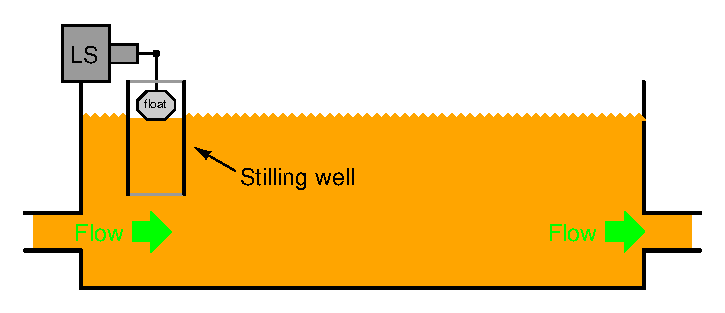
\includegraphics[width=15.5cm]{i00298x02.eps}$$

Et enkelt rørstykke fungerer ofte veldig bra som stilling well.  Man må ta forholdsregler så flottøren ikke henger seg opp inni røret, men ellers er valg og installasjon av røret normalt enkel.

%INDEX% Switch, level: used with stilling well

%(END_NOTES)
